\documentclass[9pt, a4paper]{report}
%---------------------------------------------------------------------



\usepackage[utf8]{inputenc}

\usepackage{booktabs}
\usepackage[table,xcdraw]{xcolor}


\usepackage{amsfonts}
\usepackage[english]{babel}
\usepackage[toc,page]{appendix}
\usepackage{graphicx}
\usepackage{multicol}
\usepackage{amsmath}
\usepackage{csquotes}
\usepackage{listings}
\usepackage{xcolor}
\usepackage[
backend=biber,
style=alphabetic,
sorting=ynt
]{biblatex}
\addbibresource{sample.bib}

\addtolength{\textwidth}{2in}
\addtolength{\textheight}{2in}
\addtolength{\oddsidemargin}{-1in}
\addtolength{\topmargin}{-1in}
\setlength\parindent{0pt}
%\usepackage{showframe}



\definecolor{codegreen}{rgb}{0,0.6,0}
\definecolor{codegray}{rgb}{0.5,0.5,0.5}
\definecolor{codepurple}{rgb}{0.58,0,0.82}
\definecolor{backcolour}{rgb}{0.95,0.95,0.92}

\lstdefinestyle{mystylePython}{
    backgroundcolor=\color{backcolour},   
    commentstyle=\color{codegreen},
    keywordstyle=\color{magenta},
    numberstyle=\tiny\color{codegray},
    stringstyle=\color{codepurple},
    basicstyle=\ttfamily\footnotesize,
    breakatwhitespace=false,         
    breaklines=true,                 
    captionpos=b,                    
    keepspaces=true,                 
    numbers=left,                    
    numbersep=5pt,                  
    showspaces=false,                
    showstringspaces=false,
    showtabs=false,                  
    tabsize=2
}
%---------------------------------------------------------------------

\begin{document}
\lstset{style=mystylePython}

\begin{titlepage}
    \begin{center}
        \vspace*{0.5in}
        
        \Huge
        \textbf{Modeling Chaos}
        
        Study and Simulation 
        
        of Bifurcation Systems
        
        
        \vspace*{0.7in}
        \includegraphics[width=0.6\textwidth]{Images/sulogo.png}
        
        
        \vspace*{0.5in}
        \LARGE
        \textbf{967869}
        
        \vspace*{0.2in}
        College of Science
        
        Swansea University
        
        
        
        \vfill
        \normalsize
        \begin{multicols}{2}
        Department of Physics
        
        \columnbreak
        
        $19^{th}$ March 2020
        \end{multicols}
    \end{center}
    \hrule
    
    
    \begin{abstract}
    \begin{center}
        The purpose of this work is to present the reader with an introduction to 
        linear chaotic systems. We conduct a study of deterministic chaos, proving that the one-dimensional map
        $f^{n+1}(x_n)\;=\;\mu\; x_n\; (1\;-\;x_n)$
        meets the requirements for a chaotic system defined by Devaney. Further into the work we obtain Feigenbaums constant
        using 3 different methods, with the best value obtained being $\delta = 4.6692016$. The data has been generated using
        independently written software. The software utilises techniques from multiprocessing in order to decrease data processing
        time, thus allowing for more computationally demanding tasks to be attempted.
    \end{center}
    \end{abstract}
    
    
    
\end{titlepage}

\tableofcontents
\clearpage
%---------------------------------------------------------------------

\chapter{Introduction}
\section{Chaos as a concept}
\vspace{0.3in}
\begin{center}
    \textbf{Chaos}

    \textit{"A state of total confusion with no order."}
\end{center}

This is the definition of Chaos given by the Cambridge Dictionary, and
a perfect description of the initial impressions one has observing such a system.\\
Yet physical systems like the double pendulum, vibrating objects, 
rotating or heated fluids, the motion of a group of celestial objects and dripping faucets
are deterministic in nature and can be derived from Newtons laws \cite{baker}.\\
Why is it then that we describe them as "total confusion"? To answer this question we look at
the definition to a Chaotic System given by Devaney \cite{devaney}:

\begin{center}
    Let $X$ be a metric space. A continuous map $f:\; X\to X$ is said to be
    chaotic on $X$ if:
\end{center}   

\begin{enumerate}
    \item $f$ is transitive,
    \item the periodic points of $f$ are dense in $X$,
    \item $f$ has sensitive dependence on initial conditions.
\end{enumerate}

Each of the three conditions is assured by the existences of the other two \cite{banks}, \cite{crannell}.\\
All three are listed for historical reasons and for the strength of the definition, but 
for practical purposes if two are demonstrated to be valid for a system we will
consider it chaotic.\\
The last condition is perhaps most intuitive. Imagine two systems, one of which starting with
slightly different initial conditions to the other. For non-chaotic systems this difference will 
grow linearly with time. The difference between chaotic systems, however, grows \textit{exponentially}
leading to dissimilar behavior very quickly. \\
Elaborating on the $1^{st}$ condition. A continuous map or in our case, a dynamical system
$f:\; X\to X$ is said to be transitive if, for any pair $U, V$ of nonempty open subsets of $X$
there exists some positive number of applications $n\geq 0$ of the map $f$ such that
$f^n(U)\cap V \neq \emptyset$. \cite{erdmann} \\
In Layman's terms the above claims that through some $n$ number of applications of $f$, defined hereafter as $f^n$, we can reach any
point belonging to $X$. The $2^{nd}$ rule states that every reachable point belongs to $X$.
\paragraph{}
Chaotic systems can be generalised into two families based on the equations that describe them:\\
1. Linear\\
2. Non-linear\\
In our day to day life we predominantly encounter non-linear chaos. Systems being influenced by a myriad of unpredictable
and untrackable circumstances. In this work we will study the first kind, which will require us to observe the behaviour
of the systems in the long term. 

    

\clearpage
%---------------------------------------------------------------------

\chapter{Proof of Chaotic Behaviour}
\section{Transitivity}
For the map $f:\;X \to X$, where $f$ acts as Eq.(\ref{eq:themapf})

\begin{equation}
    \label{eq:themapf}
    f^{n+1}(x)=\mu f^n(x) \times (1-f^n(x))
\end{equation}

,transitivity means that
for the domain $X$ defined by Eq.(\ref{eq:domain}),

\begin{equation}
    \label{eq:domain}
    \{x \in \mathbb{R} \; \mid \;  0 \leq x \leq 1 \}
\end{equation}

there are some finite number of iterations $n$ that would
produce a result in the co-domain $X$ defined as Eq.(\ref{eq:domain})
,illustrated in Fig.\ref{fig:setnime}.

\begin{figure}[h]
    \centering
    \includegraphics[width=0.4\textwidth]{Images/setnime.png}
    \caption{Visualisation of $f:\;X \to X$}
    \label{fig:setnime}
\end{figure}

This implies that where $f$ behaves chaotically it will \textbf{not} converge
towards one or multiple values, but rather take up all points within 
a set. In Fig.\ref{fig:trans1} we observe how many unique values $f$ generates against $\mu$,
where $\mu$ is the Growth Rate as expressed in Eq.(\ref{eq:themapf}).

\begin{figure}[h]
    \centering
    \includegraphics[width=0.8\textwidth]{Images/trans 1.png}
    \caption{Unique values of $f$ to 5 decimal places against $\mu$ }
    \label{fig:trans1}
\end{figure}

Before counting the unique values the map generates, we let the system stabilize
running it over 2'000'000 iterations without recording anything. Then values unique to 
5 decimal places are recorded. For $0\leq \mu < 3$, $f$ converges to a single value,
then at equal intervals we observe doubling. The system converges to 2, 4, 8, 16, 32, ...,
unique values.

\begin{figure}[h]
    \centering
    \includegraphics[width=0.8\textwidth]{Images/Untitled.png}
    \caption{Unique values of $f$ to 5 decimal places against $\mu$}
    \label{fig:trans2}
\end{figure}

As we look at further values of $\mu$ (Fig.\ref{fig:trans2}), this pattern is broken.
We stop observing doubling, rather $f$ begins generating a very large amount of unique
values. When we begin recording values, we run the map over 50'000 iterations.
Out of those, for $\mu > 3.695$, approximately 40'000 are unique to 5 decimal places.
This hints that at that Growth Rate $f$ becomes Transitive, generating unique values 
and allowing for any value in the co-domain to be reached allowing enough iterations. Sec.~\ref{appendix:transitivity}\\
The exact value of $\mu$ at which Eq.(\ref{eq:themapf}) becomes Transitive is

\begin{equation}
    3.570 \pm 0.005
\end{equation}


%------------------------------------------------------------------------
\newpage
\section{Dense in $X$}
For our map - Eq.(\ref{eq:themapf}), to be Dense in $X$, means that all points
the map $f$ can generate, regardless of the number of iterations, belong to
the domain of $X$ as defined in Eq.(\ref{eq:domain}).

While Transitivity and Sensitivity to Initial Conditions generally become
true where the map $f$ is chaotic (not surprising, as we are using them as
definitions of what being chaotic is), to be Dense in $X$ is a more of a formality.
The system being Dense in the co-domain is not a good sign of whether $f$ is
chaotic or not. It simply means that the system behaves. For $\mu \in [0,\; 4]$,
$f^n (x)$ will always produce a result in the domain, regardless of how many
iterations $n$ it undergoes \cite{baker} .\\

\begin{figure}[h]
    \centering
    \includegraphics[width=0.5\textwidth]{Images/max at 0.png}
    \caption{Plot of $f^n(x)$ versus $x$ for $\mu \in [0,\; 4]$}
    \label{fig:topof0}
\end{figure}

Looking at Fig.(\ref{fig:topof0}) Sec.~\ref{appendix:maxvalue} we can conclude that Max.($f^n(x)$) lies at

\begin{equation}
    \frac{\partial (f^n(x))}{\partial x}\; = \mu (1 - 2x) = 0 
\end{equation}

Thus Max.($f^n(x)$) resides at $x = 0.5$ for all $\mu$. Using this we can rigorously redefine the domain of $\mu$.
$f^n(x) \in [0,\; 1]$; Max.($f^n(x)$) = 1. 

\begin{equation}
    MAX\,(f^n(x)) = \mu 0.5 (1 - 0.5) = \frac{\mu}{4} = 1
\end{equation}
    


Therefore $\mu = 4$ is the higher boundary, and because negative values are undesirable
$\mu = 0$ is the lower boundary.

% The author leaves this proof for 
%the more mathematically inclined readers.\\
What is important is that outside of the scope of $\mu$ defined above, the system misbehaves
generating negative values or tending to infinity. There are different maps
with similar properties, where $\mu$ belongs to a different range. For 
Eq.(\ref{eq:themapf}) we will only work with $\mu \in [0,\; 4]$, as those are the values
where chaos is possible.





%------------------------------------------------------------------------
\section{Sensitivity to Initial Conditions}
\subsection{The Lyapunov Exponent}

The Lyapunov exponent is a measure of divergence between two 
systems, $f(x)$ and $f(x+\Delta x)$, evolving from slightly 
different initial conditions. This divergence is defined to be:

\begin{equation}
\label{eq:2.1}
    f^n (x+\Delta x) - f^n (x) \approx \Delta x\, e^{\lambda n}
\end{equation}

where $n$ is the $n^{th}$ iterate - $f^n (x)$,\\ 
$\lambda$ is the Lyapunov exponent and represents the average 
rate of divergence.\\
If $\lambda$ is negative, $f^n (x)$ and $f^n (x+\Delta x)$ 
converge as $n \to \infty$.\\
If $\lambda$ is positive 
$f^n (x)$ and $f^n (x+\Delta x)$ diverge; the system 
is sensitive to initial conditions \cite{baker}.\\
To be able to enumerate $\lambda$ in later computations 
Eq.(\eqref{eq:2.1}) is rearranged as shown below.\\
Eq.(\eqref{eq:2.1}) can be written as:

\begin{equation}
    \label{eq:2.2}
    \lambda \approx \frac{1}{n} ln \left[ \frac{f^n (x+\Delta x) - f^n (x)}{\Delta x} \right] 
\end{equation}

as $\Delta x \to 0$, this equation takes the form

\begin{equation}
    \lambda \approx \frac{1}{n} ln\left| \frac{d(f^n (x))}{d x} \right| 
\end{equation}
 


Applying the chain rule to the derivative of 
the $n^{th}$ iteration and taking the limit of $n \to \infty$ gives:

\begin{equation}
    \label{eq:2.3}
    \lambda = \lim_{n\to\infty} \frac{1}{n} \sum_{i=0}^{n-1} ln|f'(x_i)|
\end{equation}
%------------------------------------------------------------------------
\subsection{Methodology and the Code}
\label{section:MethodologyAndCode}
Throughout this paper there will be several sections 
discussing the technicalities of the code used to generate
the data and graphs used in the writing of this work.
The reader should not feel obliged to read through this in detail
as the rest of the discussion will repeat any necessary information.
This section is meant for those with interest in the exact workings
of the software.
\paragraph{}
While \eqref{eq:2.3} is certainly a more mathematically rigorous 
definition of the Lyapunov exponent, \eqref{eq:2.2} has its 
"derivative" part of the equation expressed in a more code friendly
way and ultimately the equation used to obtain the Lyapunov exponent
becomes:

\begin{equation}
    \label{eq:2.4}
    \lambda = \lim_{n\to\infty} \frac{1}{n} \sum_{i=0}^{n-1} ln\left| \frac{f^n (x_i+\Delta x) - f^n (x_i)}{\Delta x} \right| 
\end{equation}

\begin{lstlisting}[language=Python, caption=Lyapunov\_Exponent.py excerpt]
def lyapunov(rate):
    """Returns Lyapunov exponent for rate over N gen."""
    function = 0.2
    g_function = function+DX
    lambda = 0

    for i in range(N):
        function = rate * function * (1 - function)
        g_function = rate * d_function * (1-g_function)

        if g_function-function == 0:
            break

        lambda += d.Decimal(abs(g_function - function) / DX).ln()

    lambda = lambda / (i + 2)
    return lambda
\end{lstlisting}

The \textbf{lyapunov} function (as seen in Listing 2.1) begins by defining two variables:

\begin{equation}
    f^0(x)=0.2\; \; \; \; \; \; ;\;f^{n+1}(x)=\mu f^n(x) \times (1-f^n(x))
\end{equation}
    
\begin{equation}
    g^0(x)=f^0(x) + \Delta x \; \; \; \; \; \; ;\;g^{n+1}(x)=\mu g^n(x) \times (1-g^n(x))
\end{equation}



\eqref{eq:2.4} Defines $\lambda$ with a limit $n \to \infty$, unfortunately
that is impractical. Rather than asking \textbf{Is it possible to generate
an infinite number of iterations?}, we should ask \textbf{When is it reasonable
to stop?}\\
To answer this question lets look at where we \textbf{have} to stop.
The standard \textit{float} has 16 decimals of precision. Importing the
\textsc{decimal} module allows pushing that to 26. Pushing that even further,
although possible, would heavily impact processing time and is therefore not 
an option for this project. Even so, if the two systems are identical up to the 
26th digit after \textbf{n} iterations, it is safe to say that they do not
exhibit sensitivity to initial conditions and are therefore not chaotic.\\
To form an idea of how many iterations it is reasonable to run (Listing 2.1) for,
we look at Fig.\ref{fig:fig1}.
\begin{figure}[h]
    \centering
    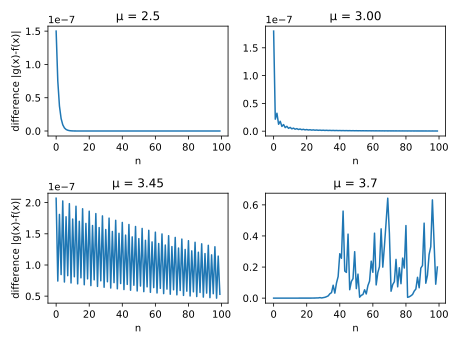
\includegraphics[width=0.8\textwidth]{Images/difference.png}
    \caption{Difference $g^n(x)-f^n(x)$ after n-th iteration.}
    \label{fig:fig1}
\end{figure}

The values for $\mu$ specify the rate of growth in $f^{n+1}(x)=\mu f^n(x) \times (1-f^n(x))$.
The paper covers these in detail later. As for now the reader needs to know that:\\
For $0<\mu<1$, $\; \;f^{n+1}(x)\;\to\;0$ as $n\to \infty$,\\
for $1<\mu<3$, $\; \;f^{n+1}(x)\;\to\;$const. as $n\to \infty,$\\
for $3<\mu<3.57$, $\; \;f^{n+1}(x)$ oscillates between several values\\
for $\approx 3.57<\mu<4$, $\; \;f^{n+1}(x)$ becomes chaotic.
\paragraph{}
Taking another look at Fig.\ref{fig:fig1}. At low values of growth -$\mu$,
it is clear that 20 iterations is enough for the two systems to become nearly identical 
up to the 26th digit. Where the systems oscillate between values, their difference 
slowly tends towards 0, which is more obvious in Fig.\ref{fig:fig2}. 2000 iterations
are not needed however, as even after 40 the difference between the two systems
is of the order $10^{-7}$, which is sufficient to declare them as not sensitive to
initial conditions.

\begin{figure}[h]
    \centering
    \includegraphics[width=0.7\textwidth]{Images/diff3.45555.png}
    \caption{Difference $g^n(x)-f^n(x)$ after n-th iteration at rate of growth $\mu=3.45$. The two systems oscillate between 4 values.}
    \label{fig:fig2}
\end{figure}

With chaotic systems, interesting behaviour occurs after the 40th 
iteration exerting the same behaviour to infinity. As such
the author finds that iterations over \textbf{n=100} are wasteful
in time, although some figures are generated with \textbf{n=1000},
where higher precision is needed.
Equipped with this knowledge we look at (Listing 2.1) again. 
Iterating $g^n(x)$ and $f^n(x)$ n=100 times, it effectively solves the equation:

\begin{equation}
    \label{eq:2.5}
    \lambda = \frac{1}{100} \sum_{i=0}^{99} ln\left| \frac{f^n (x_i+\Delta x) - f^n (x_i)}{\Delta x} \right| 
\end{equation}

Unless the difference $g^n(x)-f^n(x) = 0$, in which case it breaks the execution and solves \ref{eq:2.5}
for however many times the \textbf{for} cycle was iterated. The \textbf{lyapunov} function then returns $\lambda$ and maps it
to the corresponding rate ($\mu$) value that it was solved for. The process then start all over again,
performing the same operations for a slightly larger rate ($\mu$). In the code as seen at \ref{appendix:lyapunov}
the difference between one $\mu$ and the one for which the \textbf{lyapunov} function will be solved
thereafter is called \textsc{resolution}.

\newpage
\subsection{Lyapunov Exponent Graph and Sensitivity to Initial Conditions}

\begin{figure}[h]
    \centering
    \includegraphics[width=0.7\textwidth]{Images/Lyapunov 3.1.png}
    \caption{Lyapunov Exponent $\lambda$ as a function of the Growth Rate $\mu$ 
    for the logistic map$f^{n+1}(x)=\mu f^n(x) \times (1-f^n(x))$, 
    where $\mu \in [3,4]$. \textbf{Positive} $\lambda$ values signify
    sensitivity to initial conditions.}
    \label{fig:fig3}
\end{figure}

As discussed in \ref{section:MethodologyAndCode} \textbf{Methodology and the Code},
the Lyapunov Exponent has been solved for the logistic map 

\begin{equation}
    \label{eq:2.6}
    f^{n+1}(x)=\mu f^n(x) \times (1-f^n(x))
\end{equation}

The key variable in this equation is $\mu$. It is also referred to as the Growth Rate element,
as it controls how $f^{n+1}(x)$ grows in comparison to $f^n(x)$.\\
For $0<\mu<1$, $\; \;f^{n+1}(x)\;\to\;0$ as $n\to \infty$,\\
for $1<\mu<3$, $\; \;f^{n+1}(x)\;\to\;$const. as $n\to \infty,$\\
for $3<\mu<3.56$, $\; \;f^{n+1}(x)$ oscillates between several values\\
for $3.56<\mu<4$, $\; \;f^{n+1}(x)$ becomes chaotic.
\paragraph{}
Fig.\ref{fig:fig3} shows the Lyapunov exponent for $\mu \in [3,4]$ as that is
where the system behaves dynamically (does not settle on one value over time) 
and is of interest to us. The first thing one notices is that even where the 
system is dynamical it is not necessarily chaotic. The reason for this is
reviewed in detail in \ref{section:understandingChaos} \textbf{Towards an 
Understanding of Chaos}. $\lambda$ becomes positive for the first time at
\textbf{3.56986} as seen in fig.\ref{fig:fig4}.

\newpage
\begin{figure}[h]
    \centering
    \includegraphics[width=0.7\textwidth]{Images/Lyapunov 3.3.1.png}
    \caption{Close up of fig.\ref{fig:fig3}. Lyapunov Exponent $\lambda$ becomes positive at $\mu = 3.56986$}
    \label{fig:fig4}
\end{figure}


Obtaining the uncertainty in this value is not
a straightforward process. Traditionally uncertainty would be obtained as:


\begin{equation}
    \label{eq:2.7}
    \lambda = \frac{1}{n} \sum_{i=0}^{99} ln\left| \frac{g^n (x_i) - f^n (x_i)}{\Delta x} \right|
\end{equation}

Where, like in \ref{section:MethodologyAndCode} \textbf{Methodology and the Code}, $f^n (x_i+\Delta x) = g^n (x)$.

\begin{equation}
    \label{eq:2.8}
    d\lambda = \sqrt{ \left( \frac{d\lambda}{dg} \Delta g \right)^2 +\left(\frac{d\lambda}{df} \Delta f \right)^2} =
    \frac{1}{100} \sum_{i=0}^{99} \frac{1}{g^n (x_i) - f^n (x_i)}
\end{equation}

In this case $\Delta g$ and $\Delta f$ would be the limits of accuracy touched on in \ref{section:MethodologyAndCode},
which are 26 digits of accuracy. If one were to solve the above equation he would obtain $d\lambda \approx 10^{-21}$.
Unfortunately this is not the case. Error arises long before the program runs out of digits to store data in.
Manipulating $\Delta x$ (in $f^n (x+\Delta x)$) results in significant changes, as seen in fig.~\ref{fig:fig5}. 

\begin{figure}[h]
    \centering
    \includegraphics[width=0.7\textwidth]{Images/Lyapunov 5O.png}
    \caption{Variations of fig.\ref{fig:fig3} with different values for $\Delta x$.
    \textbf{A)}$\Delta x = 10^{-3}$, Chaos onset at $\mu = 3.45076$;
    \textbf{B)}$\Delta x = 10^{-6}$, Chaos onset at $\mu = 3.56961$;
    \textbf{C)}$\Delta x = 10^{-10}$, Chaos onset at $\mu = 3.56936$;
    \textbf{D)}$\Delta x = 10^{-16}$, Chaos onset uncertain;} 
    \label{fig:fig5}
\end{figure}

Intuition tells us that sending $\Delta x \to 0$ should result in 
more precise results. In reality there is a restriction on precision
imposed by the program used to generate these results. As discussed in
\ref{section:MethodologyAndCode} a limitation of 26 digits of accuracy
is imposed. For very small values of $\Delta x$ and non-chaotic values
of $\mu$ ($\mu \in [0,\;3.56]$), the difference $g^n (x) - f^n (x)$ 
becomes too small to be expressed within 26 digits, effectively running
for too few iterations to allow for a good estimate of $\lambda$.
The author believes this can be overcome by some clever coding which
solves the underlying problem of 

\begin{equation}
    ln\left| \frac{g^n (x) - f^n (x)}{\Delta x} \right| =\; ?\; \;;\; g^n (x) - f^n (x) = 0
\end{equation}


What does this mean for our uncertainty in $\lambda$? It is difficult to
estimate the exact effect all factors have on the value of the Lyapunov
Exponent. If we select a value for $\Delta x$ that is sufficiently small
yet large enough to allow for a satisfactory number of iterations, such as
the in fig.\ref{fig:fig3}, the value of $\mu$ at which chaos sets in is at

\begin{equation}
    3.56986 \pm 0.0005
\end{equation}
    

,which agrees with results obtained mathematically
(Chaos onset at $\mu = 3.569945672$) \cite{chaosatwolfram}.
Thus it can be concluded with 99.9$\%$c.l for values of $\mu \geq 3.7$
the map $f^{n+1}(x)=\mu f^n(x) \times (1-f^n(x))$ has sensitive dependence
on initial conditions, and thus satisfies the third and final definition
of a chaotic system.

\clearpage
%---------------------------------------------------------------------

\chapter{Towards an Understanding of Chaos}
\label{section:understandingChaos}
In this Chapter we will go towards a deeper understanding of the map $f$
and the deterministic chaos it gives rise to.
%-----------------------------------------------------------------------


\begin{figure}[h]
    \centering
    \includegraphics[width=0.7\textwidth]{Images/faigengeneral1.png}
    \caption{The Logistic Map Sec.~\ref{appendix:logicmap}. The values $f$ converges to, against Growth Rate $\mu$.
    Equilibrium achieved with 20'000 iterations}
    \label{fig:feigen1}
\end{figure}

\begin{figure}[h]
    \centering
    \includegraphics[width=0.7\textwidth]{Images/feigen3.png}
    \caption{Close up of the Logistic Map Fig.(\ref{fig:feigen1}) and illustration of
            Eq.(\ref{eq:ratio})}
    \label{fig:feigen2}
\end{figure}

When discussing a 1D map such as $f$, the Logistic Map (Fig.\ref{fig:feigen1}) presents 
the systems behaviour in the most intuitive way. At first converging 
to 0 and then to a positive number. At $\mu = 3$, the first bifurcation 
occurs - the system now oscillates between two stable states. As $\mu$
grows the number of those states becomes 4, 8, 16, 32, 64, 128, 256, ...,
until at $\mu \approx 3.570$, $f$ no longer converges and becomes
transitive. It is not unreasonable to ask: \textit{"Is the chaos we
observe just not the system having an very large number of stable states?"}.
The answer to that is a definite \textbf{No}. The difference is that 
a system with a large amount of stable states will only oscillate around those states,
while a transitive system will generate any value in the co-domain of the map
given enough iterations. What this means for us is that for a real life system described by 
a chaotic map, we cannot guess at its state out of the hypothetical $2^n$ states available,
as every state is a possible state and thus guessing becomes meaningless.
\section{Feigenbaum's number}

There is a peculiar order leading up to the point of chaos ($\mu \approx 3.570$).
Let us define the number of bifurcations with $k$, so that at $k=1$, the number of
'branches' or \textbf{Period} $= 2$.\\
Thus at $k = (2,\;3,\;4,\;k)$ the Period $= (4,\;8,\;16,\;2^k)$.
If we were to take the length of a branch (A) and divide by the length
of the branch that begins from our initial one (B) we would observe that there is 
a ratio which hold regardless of which pair we choose. That is to say, the system
 is asymptotically periodic. This is illustrated in fig.\ref{fig:feigen2}.

\begin{equation}
    \label{eq:ratio}
    Ratio\; \; \delta_k\;=\; \frac{\mu_{k+1}\;-\;\mu_{k}}{\mu_{k+2}\;-\;\mu_{k+1}}
\end{equation}

This ratio is known as Feigenbaums constant and is represented by $\delta$. There
are several different versions of $\delta$, depending on the dimension of the map,
however in this work we will focus solely on the 1D case. Feigenbaum also has a 
constant signified by $\alpha$ which has to do with the width of the branches.
In his paper from 1978 for the Journal of Statistical Physics \cite{feigenbaumconstant} he obtained 
$\delta = 4.669201609103...$. This number was later improved upon to 84 places by Briggs (1991) \cite{briggsconstant}
and again to 576 places in (1997) \cite{briggsconstant2}. Two years later Broadhurst, in an email to his friend,
defined it to 1018 places \cite{Broadhurst}.\\

Obtaining a value of our own will be the subject of the few following sections.
There are several methods one can approach this. One being simply plotting the 
Logistic Map or generating a list of the values and measuring the distance between
bifurcations. This was the method utilised by the author in the early stages of this
project, alas it is severely limited in precision due to the constraints of computer
arithmetic. The best value obtained, $\delta\; =\; 4.920$ is only a vague suggestion towards the true ratio.\\
Another method, the one utilised by Feigenbaum \cite{feigenbaumconstant}, is using
power series approximations. Below we will explore in detail a variety of different
approaches to this problem and compare results. Should the reader wish to cut to the
most accurate method, skip to the Direct Method as devised by Briggs in 1989 \cite{briggspc}.

\subsection{Looking at the Figure}
This is perhaps the least sophisticated approach. We take Fig.\ref{fig:feigen1} and
look at it really hard. Alas as we magnify the bifurcation points to pinpoint
exactly where they begin, a complication arises. As seen in Fig.(\ref{fig:trans1})
we cannot correctly determine where the branch begins due to two limitations imposed
by the capabilities of the machine and time. The first being the impossibility to fully
converge each system. A system is $f^n$ iterating continuously at a specific Growth Rate $\mu$.
The system will converge at $n \to \infty$ which is not obtainable.
The second limitation is the limitation on sample size. A sample is the number of different 
values of $\mu$ for which $f$ is iterated. If we desire a large sample size in order for
points to be denser, we limit ourselves in terms of the number of iterations $n$ we have
time to compute. As each system must go through the same number of iterations as the rest,
increasing the systems quantity lengthens computation time.

\begin{figure}[h]
    \centering
    \includegraphics[width=0.7\textwidth]{Images/feigen4.png}
    \caption{Close up of Fig.(\ref{fig:feigen1}), vertical space between the points
            is due to the system not fully converging, horizontally the data is distanced
            due to the finite number of samples in the region $\mu \in [0,\;4]$.}
    \label{fig:feigen3}
\end{figure}

Regardless with an attempt to reasonably balance sample size and iteration length we
plot Fig.(\ref{fig:feigen1}) in detail and to the best of our abilities the following data
is extracted:

% Please add the following required packages to your document preamble:
% \usepackage{booktabs}
% \usepackage{graphicx}
\begin{table}[h]
\centering
\resizebox{0.6\textwidth}{!}{%
\begin{tabular}{@{}ccccc@{}}
\toprule
$k$ & Branches $=2^k$ & $\mu_k$ & Difference $\mu_k - \mu_{k-1}$ & Ratio $\delta_k$ \\ \midrule
0   & 1               & 0       & -                              & -                \\
1   & 2               & 2.99975 & 2.99975                        & -                \\
2   & 4               & 3.44938 & 0.44963                        & 6.671597         \\
3   & 8               & 3.54076 & 0.09138                        & \textbf{4.920442}         \\
4   & 16              & 3.56439 & 0.02363                        & 3.867118         \\
5   & 32              & 3.56876 & 0.00437                        & 5.407323         \\ \bottomrule
\end{tabular}%
}
\caption{The ratio $\delta_k$ as estimated from data gathered by measuring the distance between points in Fig.(\ref{fig:feigen1}). Best estimation is
4.920 which hint towards the true value of 4.669.}
\label{tab:feigentable1}
\end{table}

While it is possible to overcome some of these obstacles by only generating samples over
the areas of interest, the true ratio $\delta$ is achieved by computing the ratio between
bifurcation points separated by infinitesimally small distances; Eq.(\ref{eq:trueratio}).
The above statement implies that there is a very harsh limit to the achievable precision
of this method.

\begin{equation}
    \label{eq:trueratio}
    \delta\; = \; \lim_{k \to \infty} \delta_k
\end{equation}

\subsection{The Fixed Point Analysis Method}

This method resolves the issue of limited precision the previous approach has
by mathematically obtaining the exact position at which the bifurcation occurs
instead of converging a system towards it. Fixed points reside within a single
state, not changing upon application of a map \cite{chaosatwolfram2};
Eq.(\ref{eq:Fixed point}).

\begin{equation}
    \label{eq:Fixed point}
    f^n(x) = x 
\end{equation}

The first stable point in the Logistic Map can be determined by Eq.(\ref{eq:Fixed point 0}).

\begin{equation}
    \label{eq:Fixed point 0}
    f^1(x_0) = x_0
\end{equation}

\begin{equation}
    \mu\,x_0\,(1-x_0)\;=\;x_0
\end{equation}
\begin{equation}
    \mu\,x_0\,(1-x_0)\,-\,x_0 \;=\;0
\end{equation}
\begin{equation}
    \mu\,x_0\,\left(x_0 - \left(\frac{1-\mu}{\mu}\right)\right)\;=\;0
\end{equation}

The solutions to this equation, $x_0 = 0$ and $x_0 = (1-\mu)/\mu$ are the 1-st order
Fixed points. The values of $\mu$ at which the stable points occur can be computed by
solving the discriminant for $\mu$. The equations below were evaluated using
Wolfram Mathematica v12.0.

\begin{equation}
Discriminant[x_0,\;\mu]
\end{equation}
\begin{equation}
Discriminant[0,\;\mu]\;=\;0
\end{equation}
\begin{equation}
Discriminant[(\mu-1)/\mu,\;\mu]\;=\;1
\end{equation}

Our 1-st order Fixed Points occur at $\mu = 0,\;1$. At this order no bifurcations
have developed. To determine the point at which the Logistic Map experiences its first
doubling we would have to solve $f^2(x_0) = x_0$.

\begin{equation}
\mu\,x_1\,(1-x_1)\;=\;x_0
\end{equation}
\begin{equation}
\mu\,(\mu\,x_0\,(1-x_0))\,(1-(\mu\,x_0\,(1-x_0)))\;=\;x_0
\end{equation}
\begin{equation}
\mu\,(\mu\,x_0\,(1-x_0))\,(1-(\mu\,x_0\,(1-x_0)))-x_0\;=\;0
\end{equation}

There are four solution's to this equation:

\begin{equation}
x_0\;=\; 0
\end{equation}
\begin{equation}
x_0\;=\; (1-\mu)/\mu
\end{equation}
\begin{equation}
x_0\;=\; \frac{\mu + \mu^2 \pm \mu \sqrt{-3 - 2 \mu + \mu^2}}{2 \mu^2}
\end{equation}

As the 2-nd order system is an iteration of the 1-st, $f(f^1(x_0))=x_0$, its solutions
include those for the 1-st order system. The last two solutions will only be real if the root is 0 or positive,
therefore we can simply solve the discriminant of what is inside it:

\begin{equation}
Discriminant[-3 - 2 \mu + \mu^2,\;\mu]\;=\;3
\end{equation}

$\mu = 3$ is therefore the point where the 1-st period doubling originates. From this point on
equations rapidly increase in size and the author will display only enough to prove his point.
We will not be solving the 3-rd order system as the solutions to that one belong to a map of higher
dimension. An oversimplified way of figuring out which order systems are of interest is that a 2-nd order
system reveals where the Logistic Map bifurcates into a total of 2 branches. A 4-th order system reveals the start
of 4 branches, 8-th order: of 8, etc. Without further delay we attempt to find our next period doubling point:
$f^4(x_0) = x_0$.

\begin{equation}
\mu\,x_3\,(1-x_3)\;=\;x_0
\end{equation}
\begin{equation}
(\mu (1 - x_0) x_0)((\mu (1 - x_0) x_0)((\mu (1 - x_0) x_0)((\mu (1 - x_0) x_0)(x_0))))-x_0\;=\;0
\end{equation}

There are 16 solutions to this, four of which are the solutions for the
1-st and 2-nd order system. The rest are roots to different powers, the contents of which are identical.

\begin{equation}
x_0\;=\sqrt{\left(\;1 + \mu^2 + ... +(-\mu^9 - 15 \mu^11 - 20 \mu^12) x_0^9 + (3 \mu^11 + 
    15 \mu^12) x_0^10 - 6 \mu^12 x_0^11 + \mu^12 x_0^12\right)}
\end{equation}

This solution is not as straightforward as the previous ones as it is dependent on $x_0$.
Setting whats inside the square root equal to 0 and solving once again for $x_0$ however gives us
the desired expressing in terms of $\mu$:

\begin{equation}
x_0\;=\;1037970703125 \mu^132 + ... + \mu^172
\end{equation}

At this point we have nearly made it. We divide all 36 terms by $\mu^{132}$ which is the one with to the smallest power.

\begin{equation}
\frac{(-5 - 2 \mu + \mu^2)^2 (5 - 4 \mu + 6 \mu^2 - 4 \mu^3 + \mu^4)^3 (-135 - 54 \mu - 
   9 \mu^2 + 28 \mu^3 + 3 \mu^4 - 6 \mu^5 + \mu^6)^4}{\mu^{132}}
\end{equation}

We take the discriminant of the numerator as that is what interests us:

\begin{equation}
Discriminant[(-5 - 2 \mu +......+ \mu^6)^4,\;\mu]\;=\;1+\sqrt{6}\;=\;3.4495, 
\end{equation}

There are multiple other solutions to the Discriminant, however most are not of interest to us
as they are either imaginary, or negative. There are two legitimate solutions, the one above and
$\mu = 3.9601$ which is the start of 4 branches at the end of one of the islands of non-chaotic behaviour
as seen in Fig.(\ref{fig:feigen2}).

\paragraph{}

Unfortunately we have hit yet another roadblock. The next Fixed point at $f^8(x_0) = x_0$ has
256 ($2^8$) solutions for $x_0$ meaning that many of the polynomials will be above 200-th order.
The author believes computation time for the above to range between several hours to a few days depending on 
the machine its being solved on. One thing is certain and it is that this method is no longer viable.

% Please add the following required packages to your document preamble:
% \usepackage{booktabs}
% \usepackage{graphicx}
\begin{table}[h]
\centering
\resizebox{0.6\textwidth}{!}{%
\begin{tabular}{@{}cccccc@{}}
\toprule
Order of fixed point & $k$ & Branches $=2^k$ & $\mu_k$ & Difference $\mu_k - \mu_{k-1}$ & Ratio $\delta_k$ \\ \midrule
1                    & 0   & 1               & 0       & -                              & -                \\
2                    & 1   & 2               & 3       & 3                              & -                \\
4                    & 2   & 4               & 3.44949 & 0.44994                        & 6.674            \\ \bottomrule
\end{tabular}%
}
\caption{The ratio $\delta_k$ as estimated from data gathered by computing fixed points}
\label{tab:feigentable2}
\end{table}

While we have figured out the points to considerable accuracy, they are so early in the series that the only
ratio $\delta = 6.674$ we are able to obtain is far from the true value.

\subsection{The Direct Method}

In the family of functions $f:\; X\to X$, so far we have been looking strictly at the map
$f^{n+1}(x_n) = \mu x_n (1 - x_n)$. There are however maps with equivalent properties and to make things
easier for ourselves we will be using one of them for this method rather than the one studied up to this point.
The reason this map is simpler is that its derivative $\partial / \partial \mu$, has an independent constant allowing
us to set variables to 0.\\
The map in question is:

\begin{equation}
    h^{n+1}(x_n) = \mu - x_n^2
\end{equation}

Similarly to how we proved our map is dense in X in Par.\textbf{2.2} we will utilise those techniques
to study the parameters of the new system.The domain of $X$ is

\begin{equation}
\{x \in \mathbb{R} \; \mid \;  -2 \leq x \leq 2 \}
\end{equation}

Max($h^{n+1}(x_n)$) lies at $x_n = 0$

\begin{equation}
\frac{h^{n+1}(x_n)}{x_n} = - 2 x_n = 0 
\end{equation}

From Eq.(\ref{eq:hofmu}) we conclude that the range of the Growth Rate is $\mu \in [0,\;2]$

\begin{equation}
    \label{eq:hofmu}
    Max(h^{n+1}(x_n)) = 2 = \mu - 0^2 = \mu 
\end{equation}

We now push the following notion: Let $\mu_k^i$ be a point at which the $i^{th}$ period doubling has occurred:
the system has stabilised into $2^i$ branches. Further let us define a super-stable point $\mu^i$ as the exact value
at which the $2^i$ branches occur. We can think of the points we obtained in Sec.~(\textbf{3.1.2}) as super-stable.
Furthermore we define Feigenbaums constants true value as Eq.(\ref{eq:trueself}).

\begin{equation}
    \label{eq:trueself}
    \delta = \lim_{i \to \infty} \left( \frac{\mu^{i-1}-\mu^{i-2}}{\mu^{i}-\mu^{i-1}} = \delta^i \right)
\end{equation}

\begin{equation}
    \label{eq:trueself2}
    \delta^i = \lim_{k \to \infty} \left( \frac{\mu_{k-1}^{i}-\mu_{k-2}^{i}}{\mu_{k}^{i}-\mu_{k-2}^{i}} = \delta_k \right)
\end{equation}

What we are doing is we are taking some points $\mu_k^i$ at which we are certain a period doubling has already occurred
then we iterate polynomials which are stable at 0, similarly to our approach in the previous section. The difference
being that in our previous approach we stabilised the polynomial by equating to 0 and attempted to obtain the exact position
with "one" calculation. While with this method we approach $\mu^i$ from some stable point between $\mu^i$ and $\mu^{i+1}$; \cite{briggspc}.
\paragraph{}
Polynomials are iterated similarly to $h$, however they are a function of $\mu$.

\begin{equation}
p_k(\mu) = \mu - [p_{k-1}(\mu)]^2
\end{equation}
\begin{equation}
p_0(\mu) = 0 
\end{equation}

Iff $p_k(\mu) = 0$, $h_{\mu}$ has a super-stable point from which $2^k$ branches originate.\\
Rearranging Eq.(\ref{eq:trueself2}) we obtain an equation for $\mu_k$:

\begin{equation}
    \label{eq:trueself3}
    \mu^{i} = \mu^{i-1} + \frac{ \mu^{i-1} -\mu^{i-2}}{\delta^i}  
\end{equation}

\begin{equation}
    \label{eq:trueself4}
    \mu_{k+1}^{i} = \mu_{k}^{i} + \frac{ p_{k}(\mu_{k}^{i}) }{ p_{k}'(\mu_{k}^{i})}  
\end{equation}

\begin{equation}
    \label{eq:trueself5}
    p_{k}'(\mu_{k}^{i}) =  \frac{\partial \left( p_{k}(\mu_{k}^{i})\right)}{\partial \mu} = 1 - 2\, p_{k-1}'\, p_{k-1}
\end{equation}

\begin{equation}
    \label{eq:trueself6}
    \mu^i = \lim_{k \to \infty} \mu_k^i
\end{equation}

Applying the above with Eq.(\ref{eq:trueself}) allows us to obtain Feigenbaums constant with increasing accuracy.
Eq.(\ref{eq:trueself3}) estimates the position of the $i^{th}$ super-stable point. Then the value of that point is refined
by iterating Eq.(\ref{eq:trueself4}), where the derivative of the polynomial with respect to $\mu$ is defined in Eq.(\ref{eq:trueself5}).
Before we attempt to estimate the following super-stable point, a new improved estimate for $\delta$ is obtained through Eq.(\ref{eq:trueself}),
allowing the next super-stable point to be obtained to greater accuracy. The whole process seems to increase precision linearly with 
every two iteration producing another true digit \cite{rosetacode}.

\newpage
\subsubsection{The Code}

\begin{lstlisting}[language=Python, caption=Code approximating Feigenbaums constant]
mu1 = 1.0           # This is Growth rate mu^(i-1)
mu2 = 0.0           # mu^(i-2)
f = 4.92           # Best approx. of Feigenbaums constant

for i in range(2, max_it + 1):
    mu = mu1 + (mu1 - mu2) / f   # mu is mu^(i)
    for k in range(1, max_it_k + 1):
        p = 0.0
        dp = 0.0
        for n in range(1, (1 << i) + 1):
            dp = 1.0 - 2.0 * dp * p
            p = mu - p**2
        mu = mu - p / dp
    f = (mu1 - mu2) / (mu - mu1)

    mu2 = mu1
    mu1 = muue. 
\end{lstlisting}

The Code utilizes the method developed by Briggs \cite{briggspc}, and its core is inspired by an anonymous contributor at
RosetaCode.org \cite{rosetacode}.\\

\begin{figure}[h]
    \centering
    \includegraphics[width=0.6\textwidth]{Images/feigen5.png}
    \caption{Branch Plot of the continuous map $f^{n+1}(x_n) = \mu - x_n^2$ belonging to the family $f:\; X\to X$}
    \label{fig:feigen5}
\end{figure}

On lines \texttt{1} and \texttt{2} we define the first two bifurcation points: $\mu^{i-2 = 0} = 0$ and $\mu^{i-1 = 1} = 1$.
$\mu^{0} = 0$ is trivial, however notice that $\mu^{1} = 1$ is a rough estimate. From Fig.(\ref{fig:feigen5}) we see
that the first period doubling beings at $\mu^1 \approx 0.75$ region, however we want to choose a stable point between
$\mu^{1}$ and $\mu^{2}$, thus we set $\mu^{1} = 1$.\\
As we enter the first \texttt{for} cycle, we solve Eq.(\ref{eq:trueself3}) on line \texttt{6}. Using this newly obtained
estimate for $\mu^3$ we iterate Eq.(\ref{eq:trueself4}) which results in $\mu^3$ converging towards its true value as
per Eq.(\ref{eq:trueself6}). Now that we have obtained a good estimate for our first three values for $\mu$ we reevaluate
the Feigenbaum constant on line \texttt{14}. Before we begin the process anew all values for mu get shifted to the right:
$\mu^{i-2} = \mu^{i-1}$, $\mu^{i-1} = \mu^{i}$. This method is mostly limited by the precision of the calculations. Without
additional improvements to the code, meaning 16 digits of accuracy with Python, one begins diverging from the Feigenbaum
constant after roughly 15 \texttt{i} iterations. This is of course dependant on the number of iterations we choose to 
complete for \texttt{k}, however it itself requires digits of precision. Overall there are many ways one can manipulate the
code to obtain better results, if one is ready to wait during the increased computation time. Sec.~\ref{appendix:feigenconst}

\subsubsection{Feigenbaums Constant - The Closest Estimate}

% Please add the following required packages to your document preamble:
% \usepackage{booktabs}
% \usepackage{graphicx}
\begin{table}[h]
\centering
\resizebox{0.4\textwidth}{!}{%
\begin{tabular}{@{}ccc@{}}
\toprule
\textbf{\texttt{i}} & \textbf{$\delta$}   & \textbf{Correct Digits} \\ \midrule
1                   & 4.92000000          & 1                       \\
2                   & 3.21851142          & 0                       \\
3                   & 4.38567760          & 1                       \\
4                   & 4.60094928          & 2                       \\
5                   & 4.65513050          & 2                       \\
6                   & 4.66611195          & 3                       \\
7                   & 4.66854858          & 4                       \\
8                   & 4.66906066          & 4                       \\
9                   & 4.66917155          & 5                       \\
10                  & 4.66919515          & 6                       \\
11                  & 4.66920019          & 6                       \\
\textbf{12}         & \textbf{4.66920169} & \textbf{8}              \\
13                  & 4.66920465          & 6                       \\
14                  & 4.66919371          & 6                       \\
15                  & 4.66926610          & 5                       \\
20                  & 4.66847161          & 0                       \\
True Value          & 4.669201609         & -                       \\\bottomrule
\end{tabular}%
}
\caption{Feigenbaums constant as computed by the Direct Method. Closest estimate obtained is $\delta = 4.66920169$.}
\label{tab:bestfeigenever}
\end{table}

The closest estimate we were able to obtain was with our final method: $\delta = 4.6692016$, Table~(\ref{tab:bestfeigenever}). 
This result has 8 digits of accuracy,
which includes numbers before the decimal separator. For practical purposes this is a satisfactory result, nevertheless 
there is allure in searching for higher and higher levels of precision. The author advises one on such a quest to further explore
the Direct Method as well as read the e-mail by Broadhurst \cite{Broadhurst} as in it he outlines the methodology used to obtain
his value, considered to be the best estimate to present day with 1018 digits.

\newpage
\section{Cobweb}

In the next few sections we will be looking to increase are intuition with chaotic systems of this type.
The next Figure (Fig.~(\ref{fig:cobweb1})) shows a plot with three lines. The blue line is a curve described by some map $f$.
The map used for Fig.~(\ref{fig:cobweb1}) is the familiar $f^{n+1}(x_n)=\mu x_n (1-x_n)$. Notice the shape recognisable as
that of a quadratic function. Feigenbaum has shown that all one dimensional maps with a single quadratic maximum bifurcate
with a period $\delta = 4.669$. \cite{feigenbaumconstant}. Naturally both maps that were explored in this work fit that description.
The second, amber line is simply an $y=x$ line. The green line appears to be "bouncing" off the previous two. Each line serves as 
a connection between two points. Disregarding the very first point, which serves to give the system its initial conditions, each point
lies on either the blue or amber line, alternating with each successive point as described in Eq.(\ref{eq:cobweb1}).
Sec.~\ref{appendix:cobweb}

\begin{equation}
    \label{eq:cobweb1}
    [f(x),\;x] \to [f(x),\;f(x)] \to [f^2(x),\;f(x)] \to [f^2(x),\;f^2(x)] \to [f^3(x),\;f^2(x)] \to etc...
\end{equation}

\begin{figure}[h]
    \centering
    \includegraphics[width=1\textwidth]{Images/cobweb4.png}
    \caption{Cobweb plot of the map $f^{n+1}(x_n)=\mu x_n (1-x_n)$; $\mu = 3$, $x_0 = 0.2$. On the leftmost figure, successive points are numbered. Both axes 
    represent some value obtainable by $f(x)$ and their range is the range of the map: $[0,\;1]$.}
    \label{fig:cobweb1}
\end{figure}

On the leftmost figure in Fig.~(\ref{fig:cobweb1}) successive points are numbered to highlight the pattern. On its right
there are figure which illustrate the continuation of the pattern. What we notice is that the points begin to converge.
Cobweb plots are very useful when it comes to studying the areas where a map converges under certain conditions. In the above
example, it converges to a single point, although that is not at all necessary. It can converge on two, four, eight or any other number
(powers of 2 only for this specific map) of values. Below in Fig.~(\ref{fig:cobweb2}) a Cobweb converging on four points can be observed.
It has been let stabilised over 1500 iterations before any values have been recorded thus making it easier for the reader to see clearly
the values of convergence.

\begin{figure}[h]
    \centering
    \includegraphics[width=0.6\textwidth]{Images/cobweb5.png}
    \caption{Cobweb plot of the map $f^{n+1}(x_n)=\mu x_n (1-x_n)$; $\mu = 3.5$, $x_0 = 0.2$. The system has undergone 1500 iterations before any values
    being recorded, and is therefore stabilised over 4 points. The reader might find it easier to decipher which those points are
    by looking solely at the $y=x$ line.}
    \label{fig:cobweb2}
\end{figure}

The really interesting thing right now is \textbf{How does a cobweb look for a chaotic system?}. Fig.~(\ref{fig:cobweb3}) shows precisely that.
On first glance it seems to be exactly what one might expect. From the 32 iterations recorded (after stabilising), 32 produce a unique point.
If we keep on plotting points however, it becomes obvious there is an order within the chaos. The system follows a specific path and it follows it,
each time with a small translation. An oversimplified analogy would be if I were to count $1,\;2,\;3,\;4,\;5 \to 1.1,\;2.1,\;3.1,\;4.1,\;5.1
\to 1.2,\;2.2,\;3.2,\;4.2,\;5.2$ etc. As the system nears its "end" where it would begin converging Fig.~(\ref{fig:cobweb3}) it always escapes
renewing the cycle, this time a little bit differently than the last.

\begin{figure}[h]
    \centering
    \includegraphics[width=0.6\textwidth]{Images/cobweb6.png}
    \caption{Cobweb plot of the map $f^{n+1}(x_n)=\mu x_n (1-x_n)$; $\mu = 4$, $x_0 = 0.2$. The system has been "stabilised" over 1500 iterations.
    From 32 recorded data points, 32 are unique.}
    \label{fig:cobweb3}
\end{figure}

\begin{figure}[h]
    \centering
    \includegraphics[width=1\textwidth]{Images/cobweb8.png}
    \caption{Left: Continuation of Fig.~(\ref{fig:cobweb3}). Right: close up of the centre where the system attempts converging.}
    \label{fig:cobweb4}
\end{figure}

\section{Fourier Transform of Time Series}

First a Time Series of a system is generated, stabilised over 10'000 iterations
and then 1000 data points are collected. Here a system is defined to be $f(x)$ for some specific Growth Rate $\mu$.
A time series for a non chaotic should should oscillate between some set number $2^k$ fixed points.
Then a fast Fourier Transform is taken of the series, with the results displayed in Fig.~(\ref{fig:4ier1}). Sec.~\ref{appendix:fourier}

\begin{figure}[h]
    \centering
    \includegraphics[width=1\textwidth]{Images/4ier5.png}
    \caption{Time Series and its Fast Fourier Transform. From top to bottom: 1)$\mu=2$, Stable points = 1, Peaks = 0;
    2)$\mu=3.2$, Stable points = 2, Peaks = 1;
    3)$\mu=3.569$, Stable points = 32, Peaks = 31;
    1)$\mu=3.8$, Stable points = none, Peaks = ?;
    }
    \label{fig:4ier1}
\end{figure}

In the non-chaotic regions the Fourier transform follows the pattern $2^k - 1$, where $k$ is the number of consecutive period doublings as 
defined in previous sections. It appears that doing the Fourier Transform of a chaotic system's time series returns random noise. In an abstract
setting as the one studied the Fourier transform does not seem to tell us anything beyond the 2 facts stated above. The reader is advised to 
perform further research before deciding on the usefulness of this method.

\section{Universality and Applications}

In this work we have encountered two maps: $f^{n+1}(x_n)=\mu x_n (1-x_n)$ and $f^{n+1}(x_n)=\mu -  x_n^2$. However bifurcation maps
can be observed for any one-dimensional maps with a single quadratic maximum. A comprehensive list can be found at \cite{wikichaoslist}.
Feigenbaums constant is believed to be transcendental and it is yet uncertain whether it is a fundamental constant like $\pi$ and $e$.
\cite{constantofnature}.

Deterministic chaos manifests itself in many forms. Although this is a Physics paper, it would be injustice to the topic to discuss
it strictly as one type of phenomenon. The more striking instances of deterministic chaos which the author encountered during his study
were "Synchronous period-doubling in flicker vision of salamander 
and man" \cite{salamander}, "Dynamics of period-doubling bifurcation to chaos in the 
spontaneous neural firing patterns" \cite{neuralfiring}, "Controlling 
cardiac chaos"\cite{cardiacchaos}, "Chaos and the Dynamics of Biological Populations"\cite{populations},
"Low dimensional chaos in cardiac tissue"\cite{cardiacchaos2}, 
"A new modified resource budget model for nonlinear dynamics in citrus production"\cite{citrusproduction} 
and "Period doubling cascade in mercury, a quantitative measurement"\cite{mercury}.





\clearpage
%---------------------------------------------------------------------

%\chapter{Universality}
%\section{equatio x}

\section{equatio y}

\section{equatio z}

\section{the family}

%\clearpage
%---------------------------------------------------------------------

%\chapter{Applications}
%\input{mazf_Applications}
%\clearpage
%---------------------------------------------------------------------
%
%\chapter{Time Series Study}
%\input{mazg_Time_series_study}
%\clearpage
%---------------------------------------------------------------------
%
%\chapter{Lyapunov Exponent}
%\input{mazh_Lyapunov_exponent}
%\clearpage
%---------------------------------------------------------------------
%

\printbibliography[
heading=bibintoc,
title={Bibliography}
]


\begin{appendices}

\chapter{The Code}
\section{Running the Code}
If this section is to be of any use to those interested in it,
some non-trivial background information has to be given if the reader
is to replicate the code.\\
The machine used to run the code has the following properties:\\
OS: Windows 10\\
IDE: Spyder 4.1.2\\
CPU: AMD Ryzen 5 2600 Six-Core Processor (2 logical cores per physical)\\
The significance of the OS is the way multiprocessing is handled by
the Python IDLE. With Windows the children of the main process are not allowed
to interact with the IDLE, thus if one wished to run the code this has to be executed
in an external terminal \cite{multistackdebug}. This can be done on Spyder by\\
\textit{Tools$\rightarrow$Preferences$\rightarrow$Run$\rightarrow$Console:Execute in an external system terminal}.
\paragraph{}
The significance of the CPU type comes from the fact the author has
utilised multiprocessing to solve the problem of long execution times
that comes with generating large amounts of data ($>$1'000'000'000 calculations required).
The software has been written to make use of 10 logical cores, and execution takes
79 minutes on average.

\newpage
\section{Lyapunov Exponent}
\label{appendix:lyapunov}
\lstinputlisting[language=Python]{Code/lyapunov_multiprocessing.py}
%---------------------------------------------------------------------

\section{Logic Map}
\label{appendix:logicmap}
\lstinputlisting[language=Python]{Code/Project.py}

\section{Cobweb}
\label{appendix:cobweb}
\lstinputlisting[language=Python]{Code/ProjectCobweb.py}

\section{Fourier}
\label{appendix:fourier}
\lstinputlisting[language=Python]{Code/ProjectFourier.py}

\section{Transitivity Bar Chart}
\label{appendix:transitivity}
\lstinputlisting[language=Python]{Code/transitivity.py}

\section{Dense in X max value graph}
\label{appendix:maxvalue}
\lstinputlisting[language=Python]{Code/max_value.py}

\section{Feigenbaums Constant}
\label{appendix:feigenconst}
\lstinputlisting[language=Python]{Code/feigenbaums_constant.py}

\end{appendices}
%---------------------------------------------------------------------

\end{document}


